\documentclass[working, oneside]{../../Preambles/tuftebook}
% Import xcolor and define some colors
\usepackage{{xcolor}}
\definecolor{{background}}{{HTML}}{{{background}}}
\definecolor{{foreground}}{{HTML}}{{{foreground}}}
\definecolor{{math}}{{HTML}}{{{color6}}}

%%%%%%%%%%%%%%%%%%%%%%%%%%%%%%%%%%%%%%%% IMPORTS %%%%%%%%%%%%%%%%%%%%%%%%%%%%%%%%%%%%%%%%
\documentclass[11pt,onesize,a4paper,titlepage]{article}

%%%%%%%%%%%%%%% Formatting %%%%%%%%%%%%%%% 
\usepackage[english]{babel}
\usepackage[utf8]{inputenc}
\usepackage{adjustbox}
\usepackage{geometry} % Margins
\usepackage{sectsty} % Custom Sections

%%%%%%%%%%%%%%% Font %%%%%%%%%%%%%%% 
\usepackage{Archivo}
\usepackage[T1]{fontenc}
\sffamily

%%%%%%%%%%%%%%% Graphics %%%%%%%%%%%%%%% 
\usepackage{fontawesome5} % Icons
\usepackage{graphicx} % Images
\usepackage[most]{tcolorbox} % Color Box
\usepackage{xcolor} % Colors
\usepackage{tikz} % For Drawing Shapes
%%%\usepackage{emoji} % For flags
\tcbuselibrary{breakable}
%%%\usepackage{academicons}

%%%%%%%%%%%%%%% Miscelanous %%%%%%%%%%%%%%% 
\usepackage{lipsum} % Lorem Ipsum
\usepackage{hyperref} % For Hyperlinks

%%%%%%%%%%%%%%% Colors %%%%%%%%%%%%%%% 
\definecolor{title}{HTML}{b5bff5} % Color of the title
\definecolor{bars}{HTML}{889af0} % Color of the title
\definecolor{backdrop}{HTML}{f2f2f2} % Color of the side column
\definecolor{lightgray}{HTML}{dfdfdf} % Color for the skill bars

%%% TU green: #639a00
%%% TU gray: #e6e6e6
%\definecolor{title}{HTML}{639a00} % Color of the title TU
%\definecolor{bars}{HTML}{889af0} % Color of the title TU

% \definecolor{backdrop}{HTML}{f2f2f2} % Color of the side column
\definecolor{backdrop}{HTML}{e6e6e6} % Color of the side column

\definecolor{subtitle}{HTML}{606060} % 


%%%%%%%%%%%%%%% Section Format %%%%%%%%%%%%%%% 
\sectionfont{                     
    \LARGE % Font size
    \sectionrule{0pt}{0pt}{-8pt}{1pt} % Rule under Section name
}

\subsectionfont{
    \Large % Font size
    \fontfamily{phv}\selectfont % Font family
    %\sectionrule{0pt}{0pt}{-8pt}{1pt} % Rule under Subsection name
    \sectionrule{5pt}{0pt}{0pt}{0pt} % Rule under Subsection name
}

%%%%%%%%%%%%%%% Margins and Headers %%%%%%%%%%%%%%%
\geometry{
  a4paper,
  left=7mm,
  right=7mm,
  bottom=10mm,
  top=10mm
}

\pagestyle{empty} % Empty Headers

\usepackage{marvosym}

% \renewcommand\qedsymbol{\CoffeeCup}

\usepackage{changepage}

\newenvironment{subexercise}[1]{%
    \begin{mdframed}[linewidth=0.5pt, linecolor=foreground, backgroundcolor=background, leftmargin=0cm, innerleftmargin=1em, innertopmargin=0pt, innerbottommargin=0pt, innerrightmargin=0pt, topline=false, rightline=false, bottomline=false]
    \par\noindent\textcolor{foreground}{\textbf{#1.}}\hspace{1em}\ignorespaces
}{%
    \par\addvspace{\baselineskip}\end{mdframed}\ignorespacesafterend
}
\newenvironment{solution}{%
    % \par\addvspace{\baselineskip}\noindent\makebox[\textwidth]{\textcolor{foreground}{\textbullet\hspace{1em}\textbullet\hspace{1em}\textbullet}}\par\addvspace{\baselineskip}
    \begin{mdframed}[linewidth=0.5pt, linecolor=foreground, backgroundcolor=background, rightmargin=0cm, innerleftmargin=0cm, innertopmargin=0pt, innerbottommargin=0pt, innerrightmargin=1em, topline=false, leftline=false, bottomline=false]
    \par\noindent\textcolor{foreground}{\textit{Solution.}}\hspace{1em}\ignorespaces
}{%
    \par\addvspace{\baselineskip}\noindent\hfill\textcolor{foreground}{\Coffeecup}\par\addvspace{\baselineskip}\end{mdframed}\ignorespacesafterend
}
% Exercise environment

\declaretheoremstyle[
    name= \textcolor{foreground}{Exercise},
    postheadspace = \newline,
    bodyfont = \normalfont\color{foreground},
    postheadhook={\textcolor{math}{\rule[.4ex]{\linewidth}{0.5pt}}\\},
    % numberwithin=chapter,
    mdframed={
        backgroundcolor = background,
        linecolor = foreground,
        linewidth = 0.5pt,
        rightline =  true,
        topline = true,
        bottomline = true,
        skipabove=20pt,
        skipbelow=20pt,
        innerleftmargin=15pt,
        innertopmargin=10pt,
        innerrightmargin=15pt,
        innerbottommargin=10pt}
    ]{exercise}
\declaretheorem[style=exercise,numbered=no]{exercise}

% \etocsetlevel{exercise}{2}

% \AtEndEnvironment{exercise}{%
%   \etoctoccontentsline{exercise}{\protect\numberline{\theexercise}}%
% }%
% \etocsetstyle{exercise}
% {}
% {}
% % this will be rendered like a non-numbered section, but we could have used
% % \numberline here also
% {\etocsavedsectiontocline{Exercise \etocnumber}{\etocpage}}
%     {}

% theorem environment

\declaretheoremstyle[
    name= \textcolor{foreground}{Theorem},
    postheadspace = \newline,
    bodyfont = \normalfont\color{foreground},
    postheadhook={\textcolor{math}{\rule[.4ex]{\linewidth}{1pt}}\\},
    mdframed={
        backgroundcolor = background,
        linecolor = foreground,
        linewidth = 1pt,
        rightline =  true,
        topline = true,
        bottomline = true,
        skipabove=20pt,
        skipbelow=20pt,
        innerleftmargin=15pt,
        innertopmargin=10pt,
        innerrightmargin=15pt,
        innerbottommargin=10pt}
    ]{theorem}
\declaretheorem[style=theorem,numbered=yes]{theorem}

\declaretheoremstyle[
    name= \textcolor{foreground}{Definition},
    postheadspace = \newline,
    bodyfont = \normalfont\color{foreground},
    postheadhook={\textcolor{math}{\rule[.4ex]{\linewidth}{1pt}}\\},
    mdframed={
        backgroundcolor = background,
        linecolor = foreground,
        linewidth = 1pt,
        rightline =  true,
        topline = true,
        bottomline = true,
        skipabove=20pt,
        skipbelow=20pt,
        innerleftmargin=15pt,
        innertopmargin=10pt,
        innerrightmargin=15pt,
        innerbottommargin=10pt}
    ]{definition}
\declaretheorem[style=definition,numbered=yes]{definition}
% Example environment

\declaretheoremstyle[
name= \quad \underline{Proof:},
     headfont = \bfseries\sffamily,
     postheadspace = \newline,
     % notebraces = \bfseries{(}{)a},
     headpunct = {},
     bodyfont = ,
     postheadhook={\textcolor{foreground}{\rule[0.4ex]{\linewidth}{0pt}}\\},
     qed=\qedsymbol,
    % spacebelow = 10pt,
    mdframed={
  backgroundcolor = background,
  linecolor = foreground,
  linewidth = 1pt,
  skipabove=10pt,
  skipbelow=10pt,
  rightline = false,
  topline = false,
  leftline = false,
  bottomline = false,
  innerleftmargin=15pt,
  innertopmargin=15pt,
  innerrightmargin=15pt,
  innerbottommargin=15pt}
]{pro}
    % \declaretheorem[style=pro,numbered=no]{Proof}

\declaretheoremstyle[
name= \quad \underline{\textcolor{foreground}{Example}},
     headfont = \bfseries\sffamily,
     postheadspace = \newline,
     % notebraces = \bfseries{(}{)a},
     headpunct = {},
     bodyfont = \normalfont\color{foreground},
     postheadhook={\textcolor{foreground}{\rule[0.4ex]{\linewidth}{0pt}}\\},
     % spacebelow = 10pt,
    mdframed={
  backgroundcolor = background,
  linecolor = foreground,
  linewidth = 1pt,
  skipabove=10pt,
  skipbelow=10pt,
  rightline = false,
  topline = false,
  leftline = false,
  bottomline = false,
  innerleftmargin=15pt,
  innertopmargin=15pt,
  innerrightmargin=15pt,
  innerbottommargin=15pt}
]{ex}
\declaretheorem[style=ex,numbered=no]{example}

\declaretheoremstyle[
     name=,
     headfont = \bfseries\sffamily,
     notebraces = \bfseries{},
     headpunct = { -},
     bodyfont = \color{foreground}\normalfont,
     % postheadhook={\textcolor{black}{\rule[.4ex]{\linewidth}{0.2pt}}\\},
    % spacebelow = 10pt,
    mdframed={
  backgroundcolor = background,
  linecolor = foreground,
  linewidth = 1pt,
  skipabove=0pt,
  skipbelow=0pt,
  innerleftmargin=10pt,
  innertopmargin=10pt,
  innerrightmargin=10pt,
  innerbottommargin=10pt,
  rightline = false,
  topline = false,
  leftline = false,
  bottomline = true}
]{subexercise}
% \declaretheorem[style=subexercise,numbered=no]{subexercise}

\declaretheoremstyle[
     name= \color{losning}Løsning,
     headfont = \bfseries\sffamily,
     notebraces = \bfseries{},
     postheadspace = \newline,
     headpunct = {:},
     bodyfont = \normalfont,
     % qed = ,
     % postheadhook={\textcolor{black}{\rule[.4ex]{\linewidth}{0.2pt}}\\},
    % spacebelow = 10pt,
    mdframed={
  backgroundcolor = background,
  linecolor = losning!75,
  linewidth = 1pt,
  skipabove=0pt,
  skipbelow=10pt,
  innerleftmargin=10pt,
  innertopmargin=10pt,
  innerrightmargin=10pt,
  innerbottommargin=10pt,
  leftline = false,
  rightline = true,
  topline = false,
  bottomline = true}
]{solution}

\newenvironment{SimpleBox}[1]{%
  \begin{mdframed}%
    \noindent\textbf{#1}\\[1ex]
}{%
  \end{mdframed}%
}


\begin{document}
\let\cleardoublepage\clearpage
\thispagestyle{fancy}
\chapter{Handin 8 - 10 ECTS}
\begin{exercise}[1]
Let $T_1, T_2, T_3$ be transactions that operate on objects M, N, O, P and Q. We now have
the following schedules:
(For brevity we use the notation $r_1\left( M \right) $ to mean that transaction $T_1$ reads object M,
$w_1\left( M \right) $ to mean transaction $T_1$ wrote to object M and $c_1$ to mean that transaction $T_1$ commits.)
\newline
For each these schedules, answer the following:
\end{exercise}
% \begin{figure}[htpb]
%     \centering
% \begin{tabular}{l|l}
% \( S_1 \) & \( r_1(M), r_2(O), w_3(P), w_1(M), r_1(O), w_2(M), r_2(N), r_2(O), w_2(N), w_3(O), \) \\
%  & \( r_2(M), w_1(N), r_1(N), r_3(P), w_1(N), r_3(N), c_1, c_2, c_3 \) \\
% \hline
% \( S_2 \) & \( r_1(Q), r_2(N), r_2(M), w_2(N), w_2(M), w_1(N), r_2(P), r_2(Q), r_3(Q), r_2(M), r_2(O), \) \\
%  & \( w_2(M), w_2(P), r_1(M), w_2(O), w_1(M), r_1(O), r_2(Q), r_3(P), r_1(M), w_3(P), \) \\
%  & \( w_1(M), r_3(M), w_1(O), r_3(M), w_1(N), r_3(O), r_3(N), r_3(O), w_3(M), c_1, c_2, c_3 \) \\
% \end{tabular}
%     \label{fig:}
% \end{figure}
\begin{subexercise}{a}
a. What does the precedence graph look like? Please remember to add labels on
the edges and to draw legibly.
\end{subexercise}
I have created the following two tables to get a better sense of what is going on, and have chosen to omit the tables provided in the exercise. I have also chosen to omit the commits at the end.

\noindent % Prevent indentation of the first minipage
\fbox{
\begin{minipage}[t]{0.48\textwidth} % Start first minipage (top aligned)
\centering % Center content within the minipage
\textbf{Schedule \( S_1 \)}
\vspace{0.5em} % Add a little vertical space
\begin{tabular}{c|c|c}
\( T_1 \) & \( T_2 \) & \( T_3 \) \\
\hline
\( r_1(M) \) & & \\
& \( r_2(O) \) & \\
& & \( w_3(P) \) \\
\( w_1(M) \) & & \\
\( r_1(O) \) & & \\
& \( w_2(M) \) & \\
& \( r_2(N) \) & \\
& \( r_2(O) \) & \\
& \( w_2(N) \) & \\
& & \( w_3(O) \) \\
& \( r_2(M) \) & \\
\( w_1(N) \) & & \\
\( r_1(N) \) & & \\
& & \( r_3(P) \) \\
\( w_1(N) \) & & \\
& & \( r_3(N) \) \\
\end{tabular}
\end{minipage}% % The '%' prevents extra space/newline between minipages
\hfill % Add flexible horizontal space between minipages
\begin{minipage}[t]{0.48\textwidth} % Start second minipage (top aligned)
\centering % Center content within the minipage
\textbf{Schedule \( S_2 \)}
\vspace{0.5em}
\begin{tabular}{c|c|c}
\( T_1 \) & \( T_2 \) & \( T_3 \) \\
\hline
\( r_1(Q) \) & & \\
& \( r_2(N) \) & \\
& \( r_2(M) \) & \\
& \( w_2(N) \) & \\
& \( w_2(M) \) & \\
\( w_1(N) \) & & \\
& \( r_2(P) \) & \\
& \( r_2(Q) \) & \\
& & \( r_3(Q) \) \\
& \( r_2(M) \) & \\
& \( r_2(O) \) & \\
& \( w_2(M) \) & \\
& \( w_2(P) \) & \\
\( r_1(M) \) & & \\
& \( w_2(O) \) & \\
\( w_1(M) \) & & \\
\( r_1(O) \) & & \\
& \( r_2(Q) \) & \\
& & \( r_3(P) \) \\
\( r_1(M) \) & & \\
& & \( w_3(P) \) \\
\( w_1(M) \) & & \\
& & \( r_3(M) \) \\
\( w_1(O) \) & & \\
& & \( r_3(M) \) \\
\( w_1(N) \) & & \\
& & \( r_3(O) \) \\
& & \( r_3(N) \) \\
& & \( r_3(O) \) \\
& & \( w_3(M) \) \\
\end{tabular}
\end{minipage}
}
\vspace{1cm}\\
\noindent
From these tables we can create precedence graphs using the rules as described by Fatemeh in the youtube video,
\begin{SimpleBox}{Precedence Graph}
For each of the transactions $T_i$ create a node. Then for each operations in the transac tions,
\begin{enumerate}
    \item if $R_i\left( X \right) $ is above $W_j\left( X \right) $ where $i\neq j$ add a directed edge from $i \to j$
    \item if $W_i\left( X \right) $ is above $R_j\left( X \right) $ where $i\neq j$ add a directed edge from $i \to j$
    \item if $W_i\left( X \right) $ is above $W_j\left( X \right) $ where $i\neq j$ add a directed edge from $i \to j$
\end{enumerate}
\end{SimpleBox}
This leads to the following precedence graphs,
\begin{figure}[htpb]
    \centering
    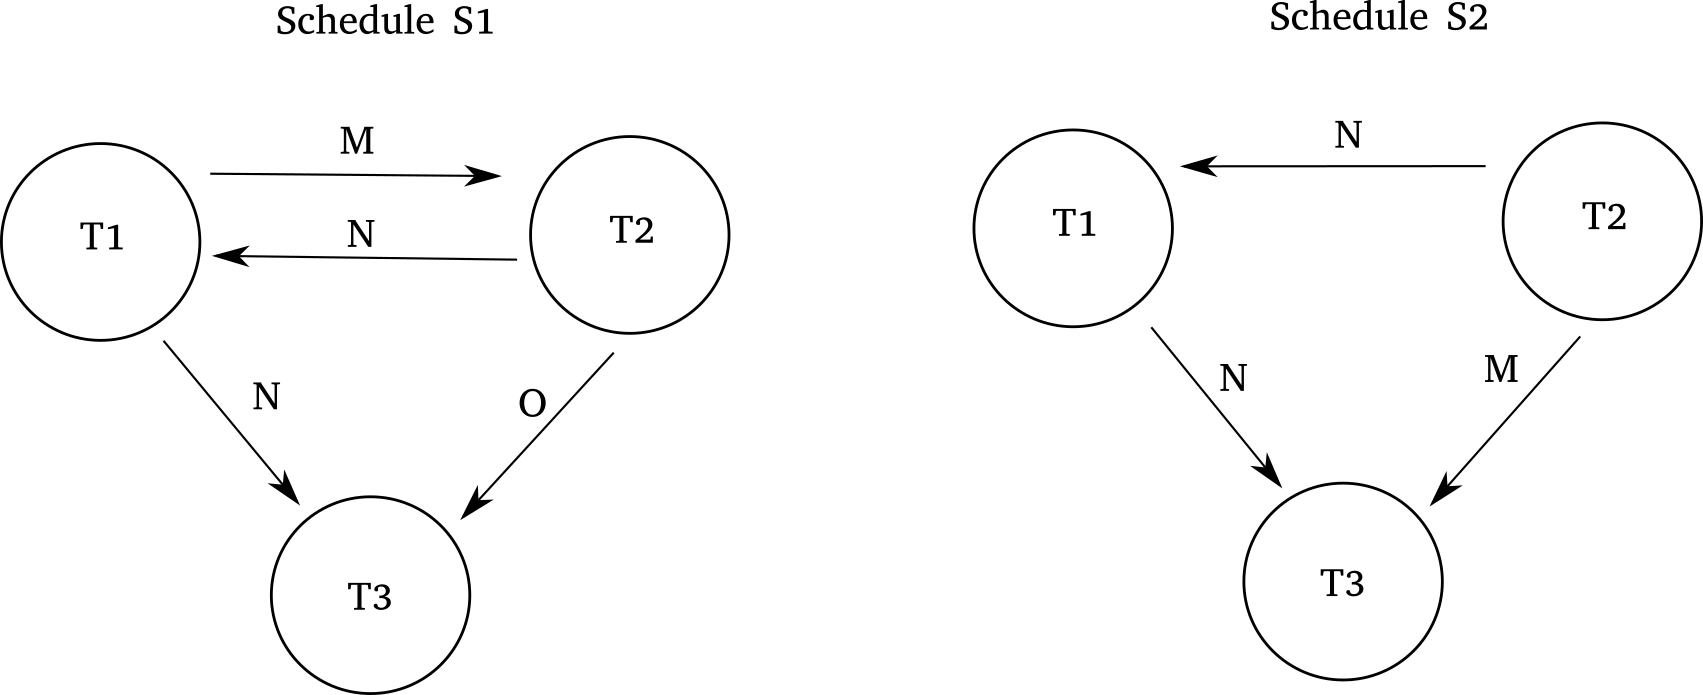
\includegraphics[width=0.8\textwidth]{afl8}
    \caption{Precendence graphs for the schedules $S_1$ and $S_2$.}
    % \label{fig:}
\end{figure}\\
Where, for example, the $N_{21}$ edge in $S_2$ comes from the read $r_2\left( N \right) $ that is then followed by a write $w_1\left( N \right) $. We could in principle have added more edges to these graphs, but they would have followed the same paths and are therefore irrelevant.
\begin{subexercise}{b}
b. Is the schedule serializable? Why so / why not?
\end{subexercise}
We can determine whether a schedule is serializable by checking for loops in the precedence graphs. Since $S_1$ has a loop, it is not serializable, whereas $S_2$ is.
\begin{subexercise}{c}
c. If yes, what is the equivalent serial schedule?
\end{subexercise}
Lets recall, that a serial schedule is one that is ordered by the transactions. That is, each transactions finishes all its operations before the next one begins. Looking at the precende graph, its clear that the order for $S_2$ should be $T_2 \to  T_1 \to T_3$
\begin{subexercise}{d}
d. Is it possible for this schedule to have been produced by 2PL? If so, expand the
schedule with the acquisition and release of locks.
\end{subexercise}
In this exercise, i'm a bit unsure whether we are supposed to use the equivalent serial schedule, or the original schedule. Let's first look at the original schedule. In 2PL, the procedure is at follows. A transaction starts by acquiring locks, does all it's operations, and then releases the locks. It is not allowed to acquire - release - acquire. In other words, once it has entered the shrinking phase, it can not begin to grow again. Let's check whether the original $S_2$ satisfies this. We can take a look at the following sequence,
\[
r_2\left( N \right) , \ldots , W_1\left( N \right) , r_2\left( P \right) 
.\] 
In this sequence, $T_2$ first acquires a read lock on $N$. Then $T_1$ acquires a write, which requires $T_2$ to release it's read lock. This implies that $T_1$ is now in the shrinking phase. However, $T_2$ immediately acquires a read lock on $P$ which violates 2PL. 
\\
The equivalent serial schedule, will trivially follow 2PL, as we can just acquire all required at the beginning of the transaction and then release them at the end,
\begin{exercise}[2]
Assume we have a relation Accounts(id, name, amount) which describes accounts at
a bank. Alice now wants to transfer 100kr to Bob’s account. This can be done by the
following SQL statements.
\begin{lstlisting}
UPDATE Accounts
SET amount = amount - 100
WHERE name = "Alice"
\end{lstlisting}
\begin{lstlisting}
UPDATE Accounts
SET amount = amount + 100
WHERE name = "Bob"
\end{lstlisting}
It is furthermore the time of the month where the bank calculates and adds the
interest, 2\% of the amount, to the account. Therefore, it runs the following update
on the database:
\begin{lstlisting}
UPDATE Accounts
SET amount = amount * 1.02
\end{lstlisting}
Now answer the following:
\end{exercise}
\begin{subexercise}{a}
What can be incorrect outcomes if the above SQL is not treated as ACID
transactions? Give an example of a schedule of the operations executed by the
above SQL statements that leads to an incorrect outcome.
\end{subexercise}
For this to go well, we essentially need to ensure that each of these transactions complte before the next one begins. If they are interleaved we can run into some issues, here is an example of one issue that might arise. Lets call Bob $T_2$ and the bank $T_3$. They each have to do the following operations,
\begin{align*}
    T_2: R_2\left( B \right) W_2\left( B \right)\\ 
    T_3: R_3\left( B \right) W_3\left( B \right)
.\end{align*}
Bob reads his bank account, adds 100, and then writes this new amount. The bank reads bobs bank account, multiplies by 1.02 and then writes this new amount. The problem arises, if we have the following sequence,
\[
R_3\left( B \right) R_2\left( B \right) W_2\left( B \right) W_3\left( B \right) 
.\] 
In this scenario the bank reads Bob's account before his changes and then overwrites his changes at the end. As a result, the 100kr that Bob added are lost.
\begin{subexercise}{b}
Which properties of ACID would it break? Why?
\end{subexercise}
The property that is primarily broken here is \textit{isolation}. Isolation ensures that each of the transactions dont interfere with one another, it essentially ensures that the database operations appear to be serial. In our case, the banks operations and Bobs are not isolated, which leads the bank to accidentally overwrite Bobs transfer. Note, that the precedence graph for this schedule has a loop, as we have the following sequence,
\[
R_3\left( B \right) \to W_2\left( B \right) \to W_3\left( B \right) 
.\] 
The way to fix this, would be to use locks. If we enforced 2PL, the bank would not be able to acquire a write lock on B, after it had released its read-lock when Bob began writing.
\begin{exercise}[3]
Consider the following trip description: \\\\
\textit{When Katrine took the plane to Munich, she checked in her suitcase and
got her boarding pass as usual. When at the gate, ready to board the
plane, she scans the barcode on her boarding pass. The electronic barrier
malfunctions and does not open to let her through, and when she tries to
scan at another barrier it does not let her through either as the bar code
has already been read by the system. The staff figures that this is simply a
flaw in the system, looks at her boarding pass and lets her board the plane.
Already seated in the plane, Katrine hears the pilot announce that the
departure has been delayed as they need to remove a passenger’s luggage
from the plane as the passenger did not board the plane. It is only on
arrival in Munich, when her luggage is missing, that she realises that it was
her luggage which was removed from the airplane.}\\\\
Now consider the entire trip, from Katrine entering the airport to her realizing her
luggage did not make it to Munich, from a database perspective. Think of this trip as
a transaction. Which important property is violated by the system or by the staff
working with the system?
\end{exercise}
The major problem seems to be consistency. When Kathrine scanned the barcode on her boarding pass, she is registered as having entered the barrier. However, it seems like the staff don't register this, so her luggage is removed from the plane. One part of the system has her registered as on the plane, while another doesn't and this leads to inconsistency
\end{document}
